%	% ****** Start of file MolecularSpinFlipLoss.tex ******
%
%
%

\documentclass[%
 reprint,
%superscriptaddress,
%groupedaddress,
%unsortedaddress,
%runinaddress,
%frontmatterverbose,
%preprint,
%showpacs,preprintnumbers,
%nofootinbib,
%nobibnotes,
%bibnotes,
 amsmath,amssymb,
 aps,
prl,
%pra,
%prb,
%rmp,
%prstab,
%prstper,
%floatfix,
]{revtex4-1}

\usepackage{graphicx}% Include figure files
\usepackage{dcolumn}% Align table columns on decimal point
\usepackage{bm}% bold math
\usepackage[hidelinks]{hyperref}% add hypertext capabilities
%\usepackage[mathlines]{lineno}% Enable numbering of text and display math
%\linenumbers\relax % Commence numbering lines
\usepackage{textcomp}

\usepackage{color}
\newcommand{\red}[1]{{\color{black} #1}}

% Define new commands for common phrases and standardized typesetting
\newcommand{\exmple}{This is an Example.}



\begin{document}

\title{New Strategy for Stark Deceleration}%

\author{David Reens}
\thanks{dave.reens@colorado.edu.}

\author{Hao Wu}
\author{Alexander Aeppli}
\author{Anna McAuliffe}
\author{Piotr Wcis\l o}
\author{Tim Langen}%
\altaffiliation{Present Address: 5. Physikalisches Institut and Center for Integrated Quantum Science and Technology (IQST), Universit\"at Stuttgart, Pfaffenwaldring 57, 70569 Stuttgart, Germany}

\author{Jun Ye}
\affiliation{JILA, National Institute of Standards and Technology and the University of Colorado and\\ Department of Physics, University of Colorado, Boulder, Colorado 80309-0440, USA}


\date{\today}

%%%%%%%%%%%%%%%%%%%%%
% OUTLINE 
%%%%%%%%%%%%%%%%%%%%%
% Introduction
% Effective Moving Trap
% Alternate Charging Technique
% Experimental Validation
% Further Simulation Results


%%%%%%%%%%%%%%%%%%%%%
% ABSTRACT
%%%%%%%%%%%%%%%%%%%%%
\begin{abstract}
Since its first realization, Stark deceleration has unlocked incredible new opportunities for the control of molecular beams. 
Numerous trapping and collisional studies have been performed, and several important extensions to the technique have been developed. 
Nevertheless, Stark deceleration has thus far been prevented from realizing its full potential due to significant limitations in the performance of the deceleration strategies thus far utilized.
We introduce a new strategy that offers many-fold performance improvements across all useful operating conditions for a Stark decelerator, including ten-fold increases in molecule number at trappable final velocities.
Our strategy also makes the application of Stark deceleration to less readily polarized species more feasible, and removes loss-inducing instabilities which formerly limited the viability of longer devices.
\end{abstract}

\maketitle


%%%%%%%%%%%%%%%%%%%%%%%%%%%%%%%%%
%     INTRODUCTION
%%%%%%%%%%%%%%%%%%%%%%%%%%%%%%%%%
%\section{Introduction}
Over the past two decades, Stark deceleration has enabled groundbreaking collisional~\cite{Sawyer2011,Kirste2012,Gao2018} and spectroscopic~\cite{Veldhoven2004,Hudson2006,Lev2006,Fast2018} studies of a variety of species~\cite{VanDeMeerakker2012}. 
Subsequent trap-loading greatly enhances interrogation time for such studies~\cite{Sawyer2008} and opens the door for further cooling and manipulation~\cite{Stuhl2012evap, Reens2017}. 
Alongside the history of achievements enabled by Stark deceleration runs a parallel ongoing saga surrounding their efficient operation. 
Many important steps have been made, not only in understanding the flaws of the canonical pulsed decelerator~\cite{VanDeMeerakker2006,Sawyer2008a}, but also in addressing them through the use of overtones~\cite{VanDeMeerakker2005a,Scharfenberg2009}, undertones~\cite{Zhang2016}, or even mixed phase angles~\cite{Parazzoli2009,Hou2013}. 
Even with these advances, the outstanding inefficiencies of the pulsed decelerator, particularly with regard to transverse phase stability, have motivated alternative geometries such as interspersed quadrupole focusing~\cite{Sawyer2008a} and traveling wave deceleration~\cite{Osterwalder2010,VandenBerg2014,Fabrikant2014}. 
Although traveling wave deceleration takes a strong step toward truly efficient operation, it comes with costs in system complexity. 
These costs can be partially addressed by the use of combination pulsed and traveling wave devices~\cite{Quintero-Perez2013}, or even using traveling wave geometry with pulsed electronics~\cite{Hou2016,Shyur2017}. 
Others continue to pursue brand new geometries aiming to enhance transverse acceptance without abandoning more reliable pulsed electronics~\cite{Wang2016}. 
Our strategy works with conventional geometry and electronics, but fully resolves transverse challenges and offers more than tenfold gains even at very low speeds.
%In the same spirit, we introduce here a technique that uses conventional geometry and pulsed electronics, but with charge applied in an alternative manner. 
%Our technique enables manyfold enhancements in molecule number across all final speeds, and can be implemented on existing devices with neither length increases nor complex electronics. 
%In addition, by analyzing the details of the effective moving trap generated by our alternative sequences, we demonstrate that our technique in fact improves over the performance offered by traveling wave devices, at all but the slowest speeds.

\begin{figure}[t]
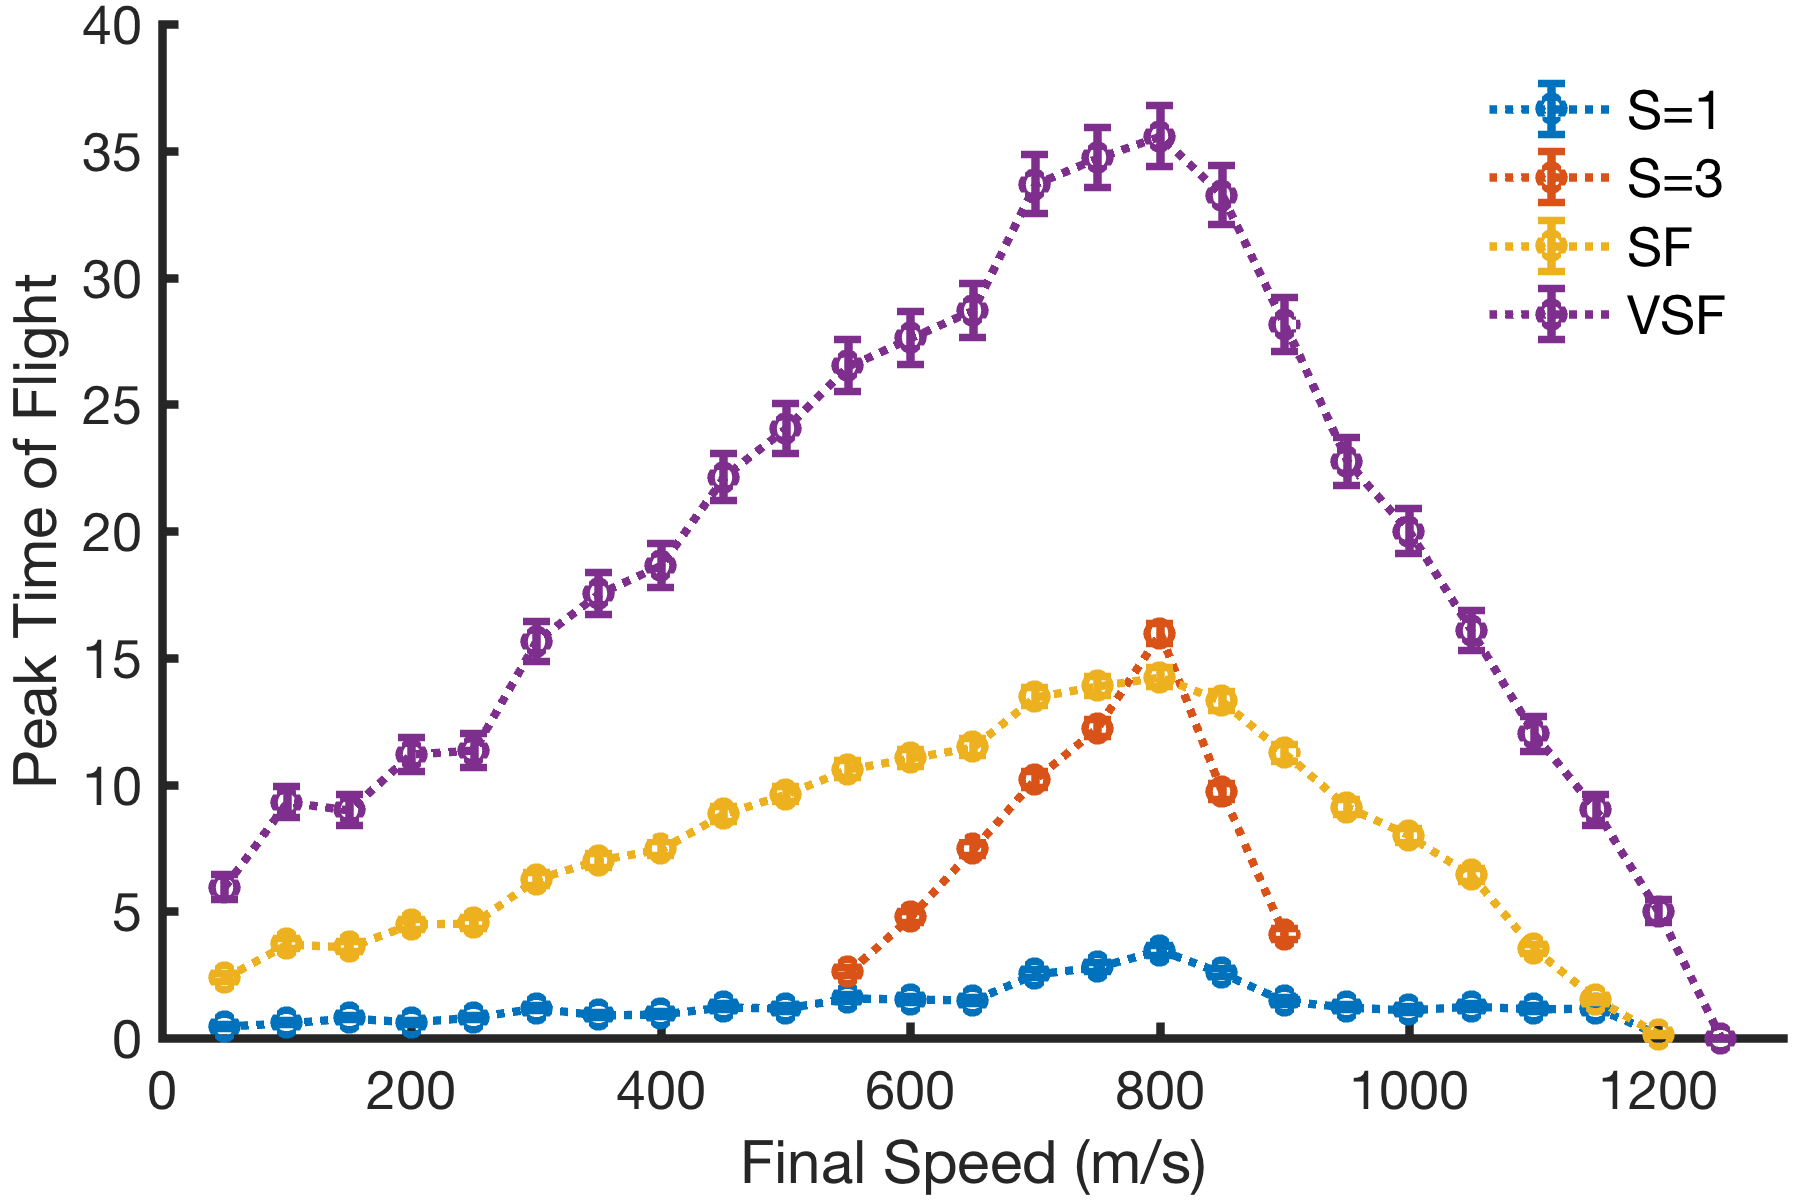
\includegraphics[width=\linewidth]{Data/Data-Figure-Final-Speed.png}%
\caption{\label{fig:alldata}
Experimental comparison of deceleration strategies. 
Data are collected with a $333$ stage decelerator and a beam of OH radicals expanded in Neon at an initial speed of $820\text{ m/s}$. 
Large gains persist at low speeds, with SF, an operating mode employing the new strategy, outperforming S\,=\,1 at $50\text{ m/s}$ elevenfold.
Larger accelerations than decelerations are possible in the device, demonstrating the increased range of SF mode.\vspace{-4mm}
}
\end{figure}


The strategy is to mix new field distributions into the deceleration process that feature strong restoring force in the transverse directions.
%Field distributions with this property include those arising from applying voltage $V$ to only one of the four distribution rods in a Stark decelerator, from applying the same voltage $V$ to both pins in a pair rather than opposite polarities, 
Depending on which field distributions are admixed, we specify several operating modes employing this strategy: focusing (F), strong focusing (SF), and very strong focusing (VSF).
The measured performance of these modes against the S\,=\,1 and S\,=\,3 operating modes which employ the conventional strategy is shown in Fig.~\ref{fig:alldata} for hydroxyl radicals, a benchmark species for Stark deceleration.
These are performed on a decelerator not previously reported, with $2$~mm pin spacing and other geometric parameters as in our earlier devices~\cite{}, but with $333$ total stages- suitable for decelerating a beam seeded in neon from $800$~m/s to rest.
F mode, which requires no wiring changes and may be immediately employed on existing devices already enhances performance by a factor of $4-8$.
With some investment in high voltage equipment, we also implement SF mode, providing an additional significant gain. %which requires a tri-state switch capable of double the usual switching frequency~\footnote{Behlke HTS-301-151-SiC, options HFB, ILC, ALL-OFF-BIPOLAR.}, so as to make use of the field distribution arising from charging both pins in a pair to the same nenzero voltage.
A comparable investment would enable VSF mode, but we do not pursue this since it is less useful for trapping, our primary emphasis, for reasons discussed further below.
The slowest speeds shown are typical in a system such as ours designed to provide molecules that are one pulse away from being trapped.
%Hold times vary from $2-4\text{ ms}$ as final speed is tuned, and thus are in agreement with the simulation results reported for $3\text{ ms}$ in Fig.~\ref{fig:efftrap}.


%\section{Alternate Charging Technique}

\begin{figure*}[t]
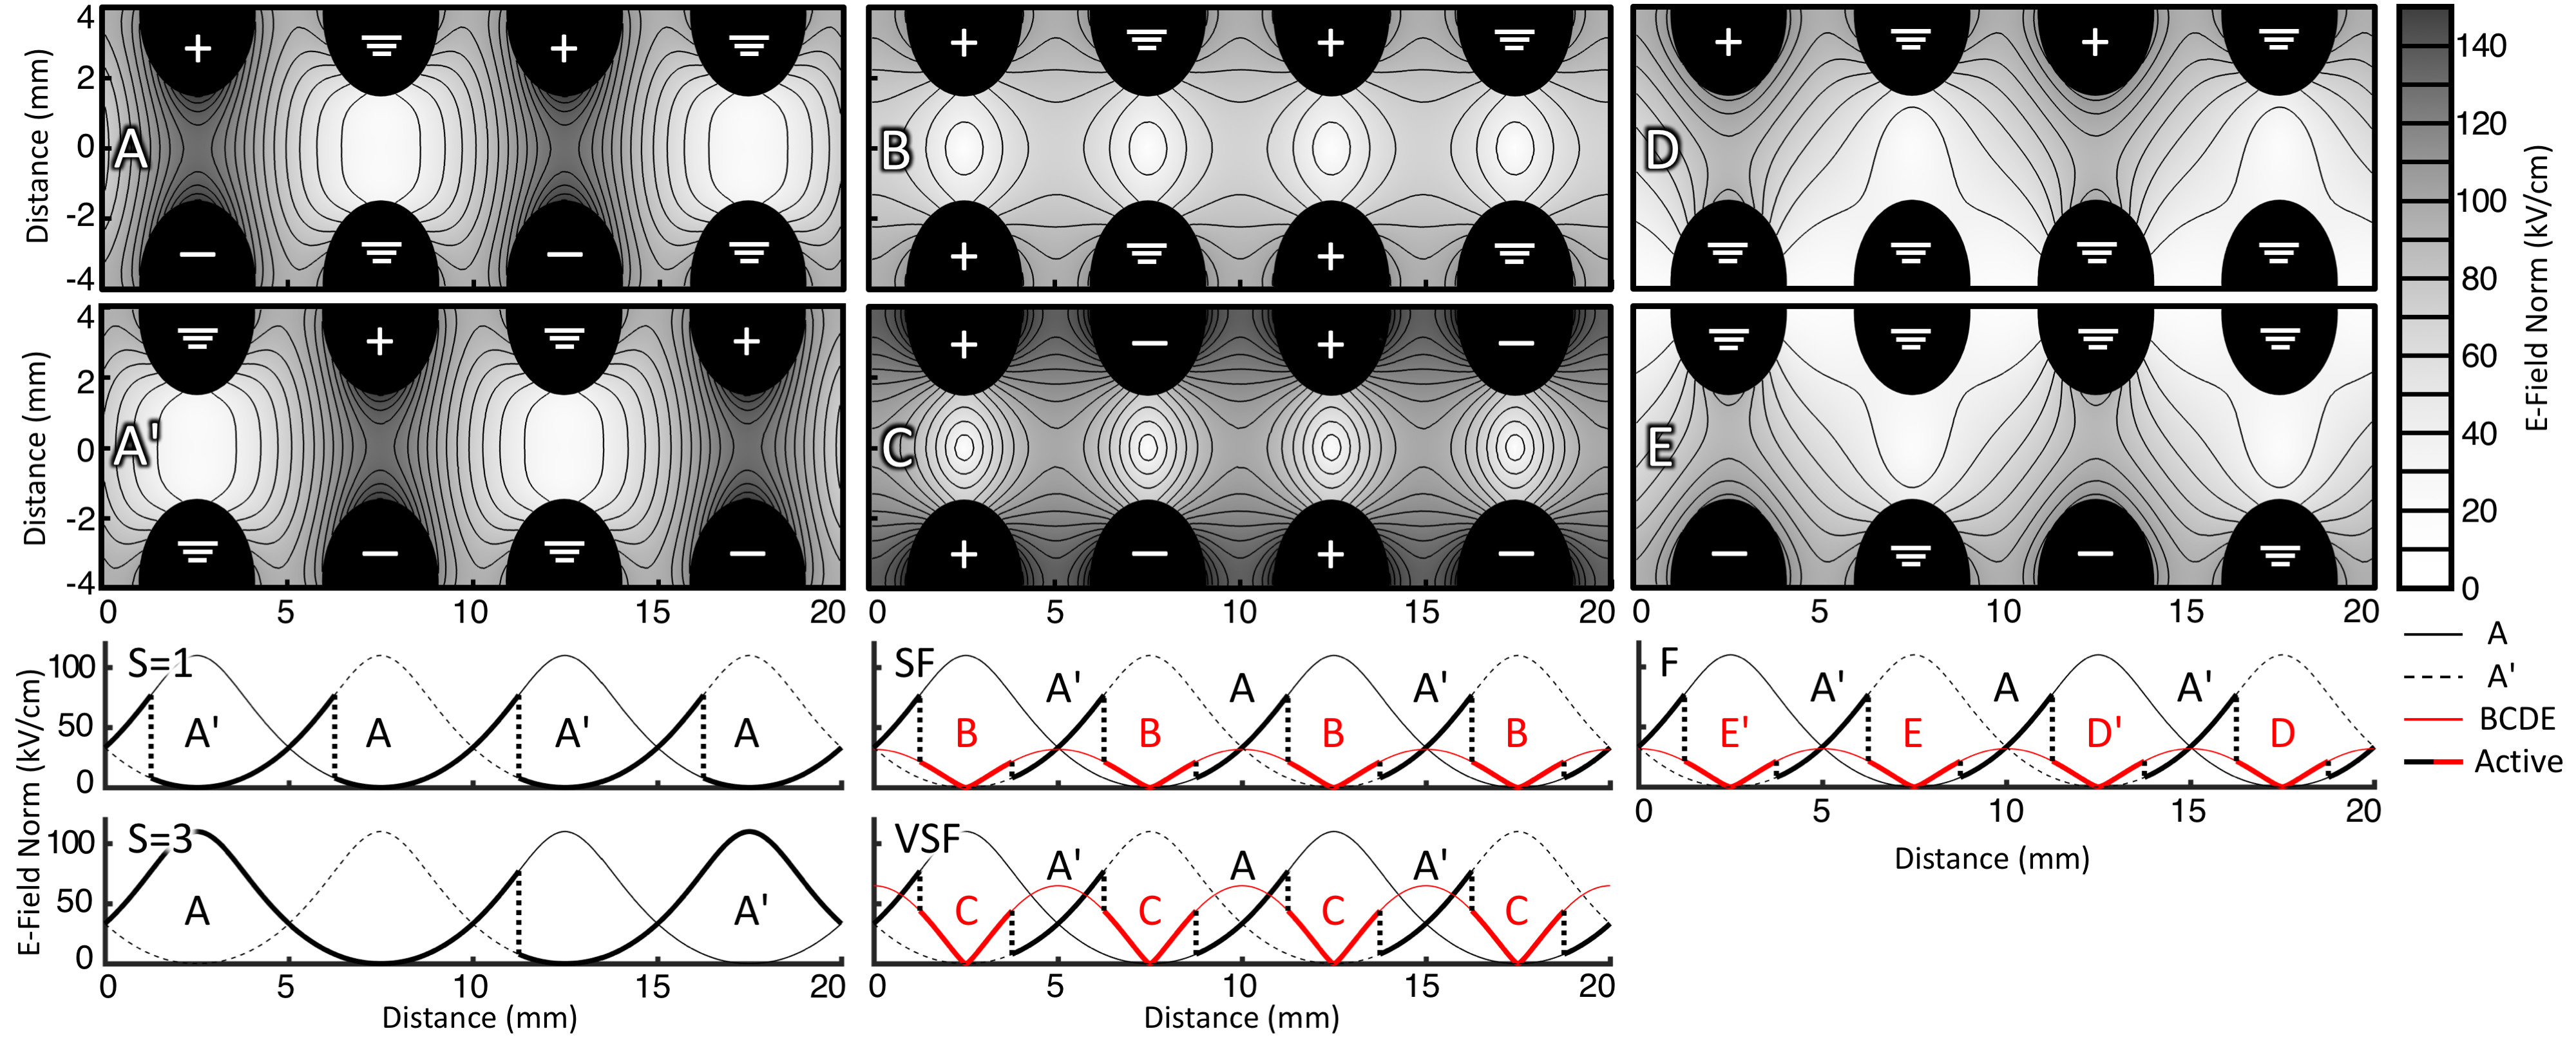
\includegraphics[width=\linewidth]{Configurations/pinpairformal6.png}%
\caption{
A new strategy for Stark deceleration, consisting of novel distributions of the electric field and operation modes which employ them. Distributions B-E feature strong transverse focusing where molecules would normally pass between grounded pin pairs. On-axis energy diagrams are shown for operation modes F, SF, and VSF which incorporate Distributions D/E, B, and C respectively. Primes indicate translation to the next pin pair. Conventional operating modes S\,=\,1,3~\cite{VanDeMeerakker2005a}, are also shown.\vspace{-4mm}
}
\label{fig:chargecartoon}
\end{figure*}

%This restoring force averages into the effective moving trap, leading to the dramatic improvements over S=1 shown in Fig.~\ref{fig:efftrap}. 
The reason for the dramatic success of this new deceleration strategy may be understood as follows.
In the conventional strategy~\cite{VanDeMeerakker2012}, molecules approach a charged pin pair, climbing a hill in potential energy. 
The hill is abruptly switched off, allowing molecules to then repeat the process without regaining that potential energy.
The abrupt switch occurs partway up the potential energy hill, so that molecules that are ahead get more energy removed, and vice versa. 
This creates a traveling potential well for the molecules, with a longitudinal restoring force towards the center of a decelerating reference frame whose deceleration is set by the chirp rate of the switching frequency.
It is customary to define an idealized ``synchronous molecule'' with zero energy with respect to this potential well, which proceeds exactly down the central axis of the decelerator and climbs each potential hill to the same position at the moment of a switching event.
In the transverse directions, restoring force is not inherited from switching events, but arises directly from the focusing properties of field distributions in the lab frame.
Pins are always charged in bipolar pairs, in which case transverse focusing occurs right between the charged pin pair, but not significantly elsewhere.
This causes molecules to experience much better transverse focusing when they are regularly sampling the focusing fields right between the charged pin-pair, which requires them to be oscillating regularly ahead and behind the synchronous molecule.

Just after the switching event, which as mentioned must happen only partway up the potential energy hill, molecules proceed through the largely field-free region between grounded pin pairs.
This region is of central importance to our new deceleration strategy.
Useful field distributions with transverse focusing in this region can be created by applying voltage in a way that is not balanced between adjacent pin pairs. 
%Once an imbalance exists, by charging up both pins in a pair to the same non-zero voltage, by only charging one pin in a pair, or even by unbalancing the decelerator power supplies~\cite{Hoekstra2018}, the field lines will run between pin-pairs. 
This imbalance causes field lines to run toward the grounded pin pair, creating a focusing 2D quadrupole structure, much like this one used intentionally for trapping and controlling spin-flip losses~\cite{Reens2017}. 
By implementing these distributions when the synchronous molecule is flying between the grounded pin pair, but retaining the use of the conventional distribution otherwise, the longitudinal behavior of the device is preserved while the transverse behavior is vastly improved.
%Regarding spin-flip losses, use of these configurations is cause for concern, but so far not a significant effect~\cite{ssm}.
\begin{figure*}[ht!]
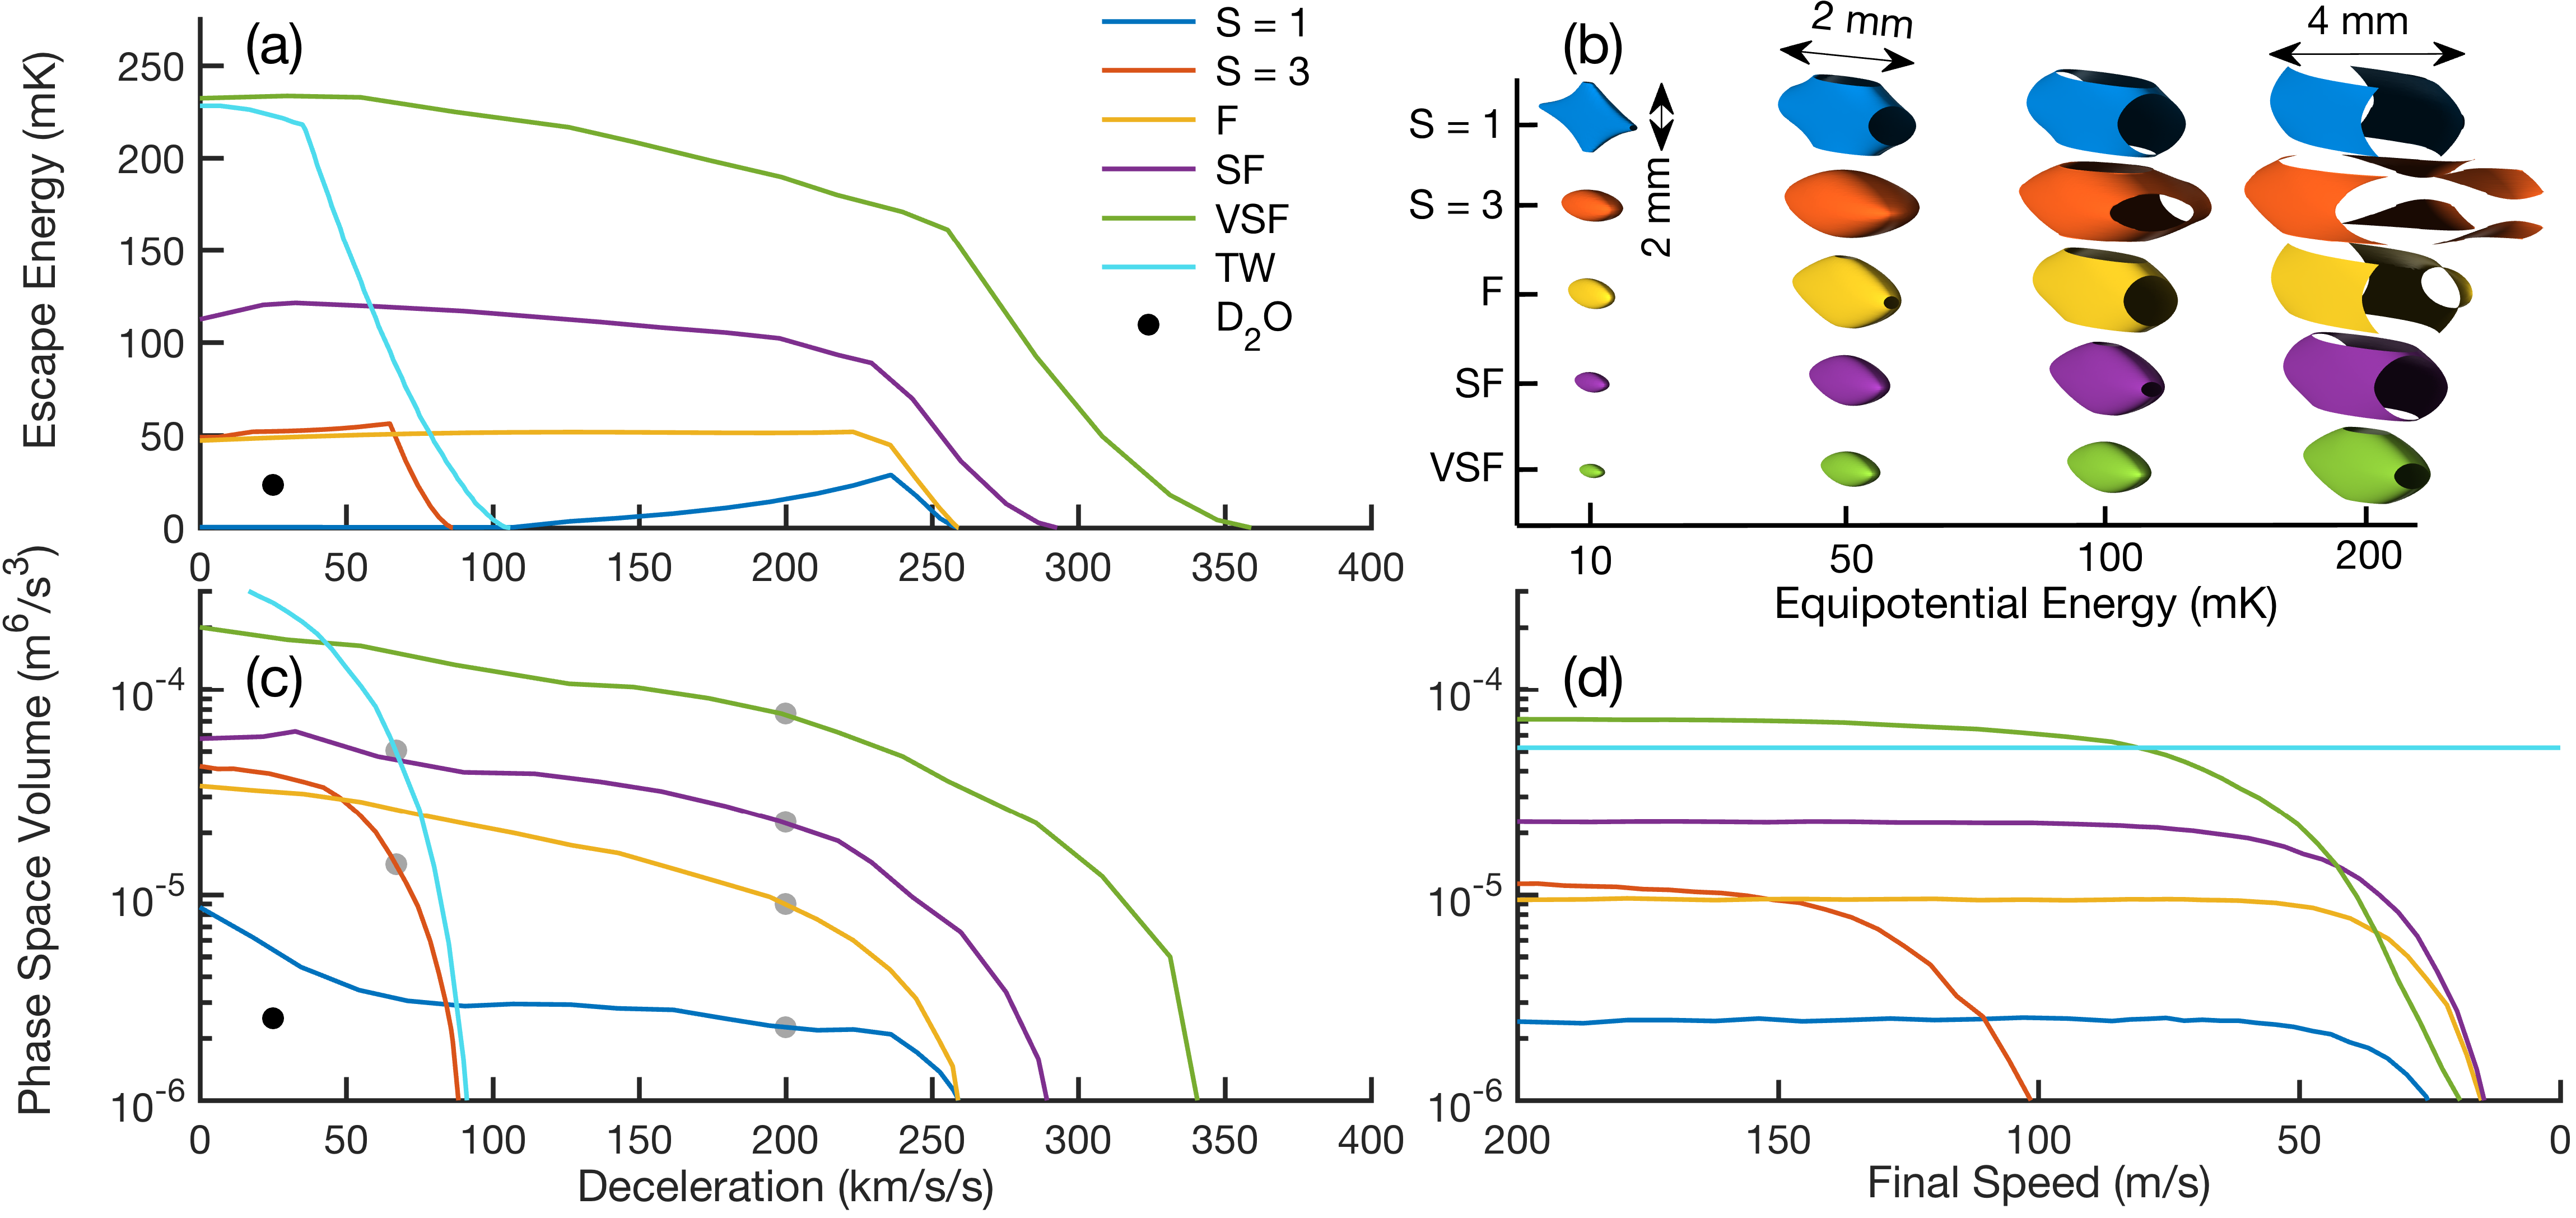
\includegraphics[trim=45 7 40 10, clip, width=\linewidth]{full-four-panel.png}%
\vspace{-5pt}
\caption{
Characterizing the moving potential well under different modes of operation. In addition to the conventional S\,=\,1 and S\,=\,3 modes, newly defined focusing (F), strong focusing (SF), and very strong focusing (VSF) modes employing the new deceleration strategy are shown. Traveling wave (TW) deceleration is also compared, assuming $10$~kV peak to peak, to our knowledge the largest voltage used to successfully decelerate to rest with a TW device. In panel (a) the well depth at the lowest point of escape is shown as a function of deceleration. Panel (b) shows equipotentials of this well; lack of closure of an equipotential equates to escape. In panel~(c) the initial phase space volume remaining within these traveling wells after a $3$~ms hold time is shown, and in panel (d) a full decelerator simulation is performed as a function of final velocities, with hold time fixed also at $3$~ms and deceleration fixed as indicated by the gray dashed lines in panel~(c). For TW a full simulation is not performed, since low speed losses are less significant, but the dashed line shows the value corresponding to $67$~km/s/s in panel (c).\vspace{-4mm}}
\label{fig:efftrap}
\end{figure*}
We identify several operational modes employing this strategy, varying according to the magnitude of their transverse focusing effects.
Utilizing the field distribution arising from charging only a single rod, something readily achievable with no change to high voltage electronics, gives rise to a focusing mode (F).
Charging two pins to the same voltage gives rise to strong focusing (SF), and charging all four pins, one pair at one voltage and the next pair at the opposite voltage, gives very strongly focusing (VSF).

%\section{The Effective Moving Trap}
In order to quantitatively analyze these operation modes, we can work in the decelerating non-inertial frame of the molecules, where a traveling potential well is generated with deceleration included as a fictitious force. 
%One of the key motivations for improvement of the conventional pulsed decelerator operation are its well-known failings as far as phase-space stability is concerned. These have been described in terms of transverse-longitudinal couplings~\cite{VanDeMeerakker2006}, small separatrix area at high phase angles~\cite{Hudson2004}, or reflection at low velocities~\cite{Sawyer2008a}. 
This approach is usually reserved for continuous deceleration schemes~\cite{Osterwalder2010,Narevicius2008}, but is equally valid for pulsed schemes provided their velocity satisfies $v/D >> f$, $D$ the stage distance and $f$ the oscillation frequency in the traveling well.
%Here $D$ is the distance between stages of the pulsed device, and $f$ is the oscillation frequency in the effective trap. 
The breakdown of this traveling potential well approximation occurs at very low speeds ($\sim\!\!50\text{ m/s}$) relative to initial beam speeds, and is discussed further below.
The traveling potential for on-axis molecules in the longitudinal direction has been discussed at length~\cite{Bethlem2000,Hudson2004}, but computation of the full 3D potential has not been reported previously.
We derive it here~\cite{ssm}, and we evaluate it numerically for various operation modes to obtain the equipotential surfaces in Fig.~\ref{fig:chargecartoon}.
For the conventional strategy and the S\,=\,1 operating mode, the traveling potential well has holes; i.e. the equipotential surfaces at very small energies with respect to the traveling potential well are not closed, enabling some molecules to escape transversely and encounter the surfaces of decelerator pins. 
Molecules moving away from the trap center along the $x$ and $y$ axes experience almost no restoring force at all. 
This can be considered the underlying reason for the transverse-longitudinal coupling problem that has been described~\cite{VanDeMeerakker2006}. 
Such couplings are in some contexts useful for maintaining ergodicity in a potential well~\cite{Surkov1996}, but with one dimension featuring a very low energy barrier, they lead to loss.

Motivated by the holes evident in S\,=\,1 mode, we introduce a new figure of merit that may be used to compare the performance of various modes of operation: the minimum depth of their traveling potential wells.
Here minimum depth refers to the smallest energy above which a molecule with that energy can find a way out of the trap.
Having a single value to characterize effective traps allows us to do so systematically across many modes and across many magnitudes of the applied deceleration, see Fig.~\ref{fig:efftrap}a. 
Remarkably, F mode offers comparable well depth to S=3, but with no sacrifice in deceleration capability. 
The SF and VSF modes make more dramatic improvements, with the latter rivaling traveling wave (TW) deceleration~\cite{Osterwalder2010}. 
Note that for SF and VSF, the transversely focusing field distributions are not utilized in a symmetric manner about the grounded pin pair as described above. 
Instead, allowing them to be used asymmetrically opens up a new degree of freedom, which we optimize so as to maximize the well depth~\cite{ssm}.

We can make further use of the traveling potential well by directly employing it to simulate the fate of particles confined for $3\text{ ms}$, the duration of a typical deceleration sequence (Fig.~\ref{fig:efftrap}b). 
The results show a very close qualitative match to the trends predicted by the minimum well depth, compare Fig.~\ref{fig:efftrap}a,b.
%The most notable exception is found in S=1 mode at low decelerations, where extremely deep holes dominate the minimum trap depth, but the small effective cross sectional area of the holes still allows molecules to survive in greater number than at higher decelerations where the minimum trap depth actually improves.
As far as the comparison with TW is concerned, it is important to point out that we use the rather small $2\text{ mm}$ pin-pair spacing and $2$x$2\text{ mm}^2$ opening area of our device, while TW devices use $4\text{ mm}$ diameter rings.
If VSF mode were used with a $3$x$3\text{ mm}^2$ device~\cite{Scharfenberg2009} or a $4$x$4\text{ mm}^2$~\cite{VandeMeerakker2005}, phase space volume would increase significantly, depending approximately on the cube of pin-pair spacing, and thus outperforming TW. 

Of course the validity of using the traveling potential well in this manner depends on the final speed after the deceleration sequence.
We study this by also performing a full Monte-Carlo simulation of the various deceleration modes, without use of the traveling well approximation.
By varying only the final speed, and keeping deceleration and run-time exactly fixed by appropriately varying initial speed and decelerator length, we obtain the results shown in Fig.~\ref{fig:efftrap}c. 
The asymptotically flat profiles at high enough speeds validate the traveling potential approach, as do the quantitative agreement between the asymptotic values and the corresponding points at $200\text{ km/s/s}$ and $67\text{ km/s/s}$ in Fig.~\ref{fig:efftrap}b. 

The beginning of the low-speed breakdown depends on the intended use of the decelerator, and especially how far the molecules will be expected to travel unguided afterwards. 
In Fig.~\ref{fig:efftrap}c, the molecules still confined within a $3\text{ mm}$ diameter circle after $5\text{ mm}$ free flight after the end of the sequence are shown. 
This is a conservative representation of what is required for trap-loading, but for collisional experiments a larger flight distance may be required.
Note how F and SF cut off at even lower speeds than S\,=\,1, but VSF cuts higher. 
This can be attributed to the fact that VSF actually features an increased transverse trap frequency relative to the others, while F and SF improve over S\,=\,1 mostly by hole mitigation, not by increasing the transverse confinement strength of the well.
VSF mode may be especially useful for trap loading in combination with a TW device as in~\cite{Quintero-Perez2013}.

%\begin{figure}[t]
%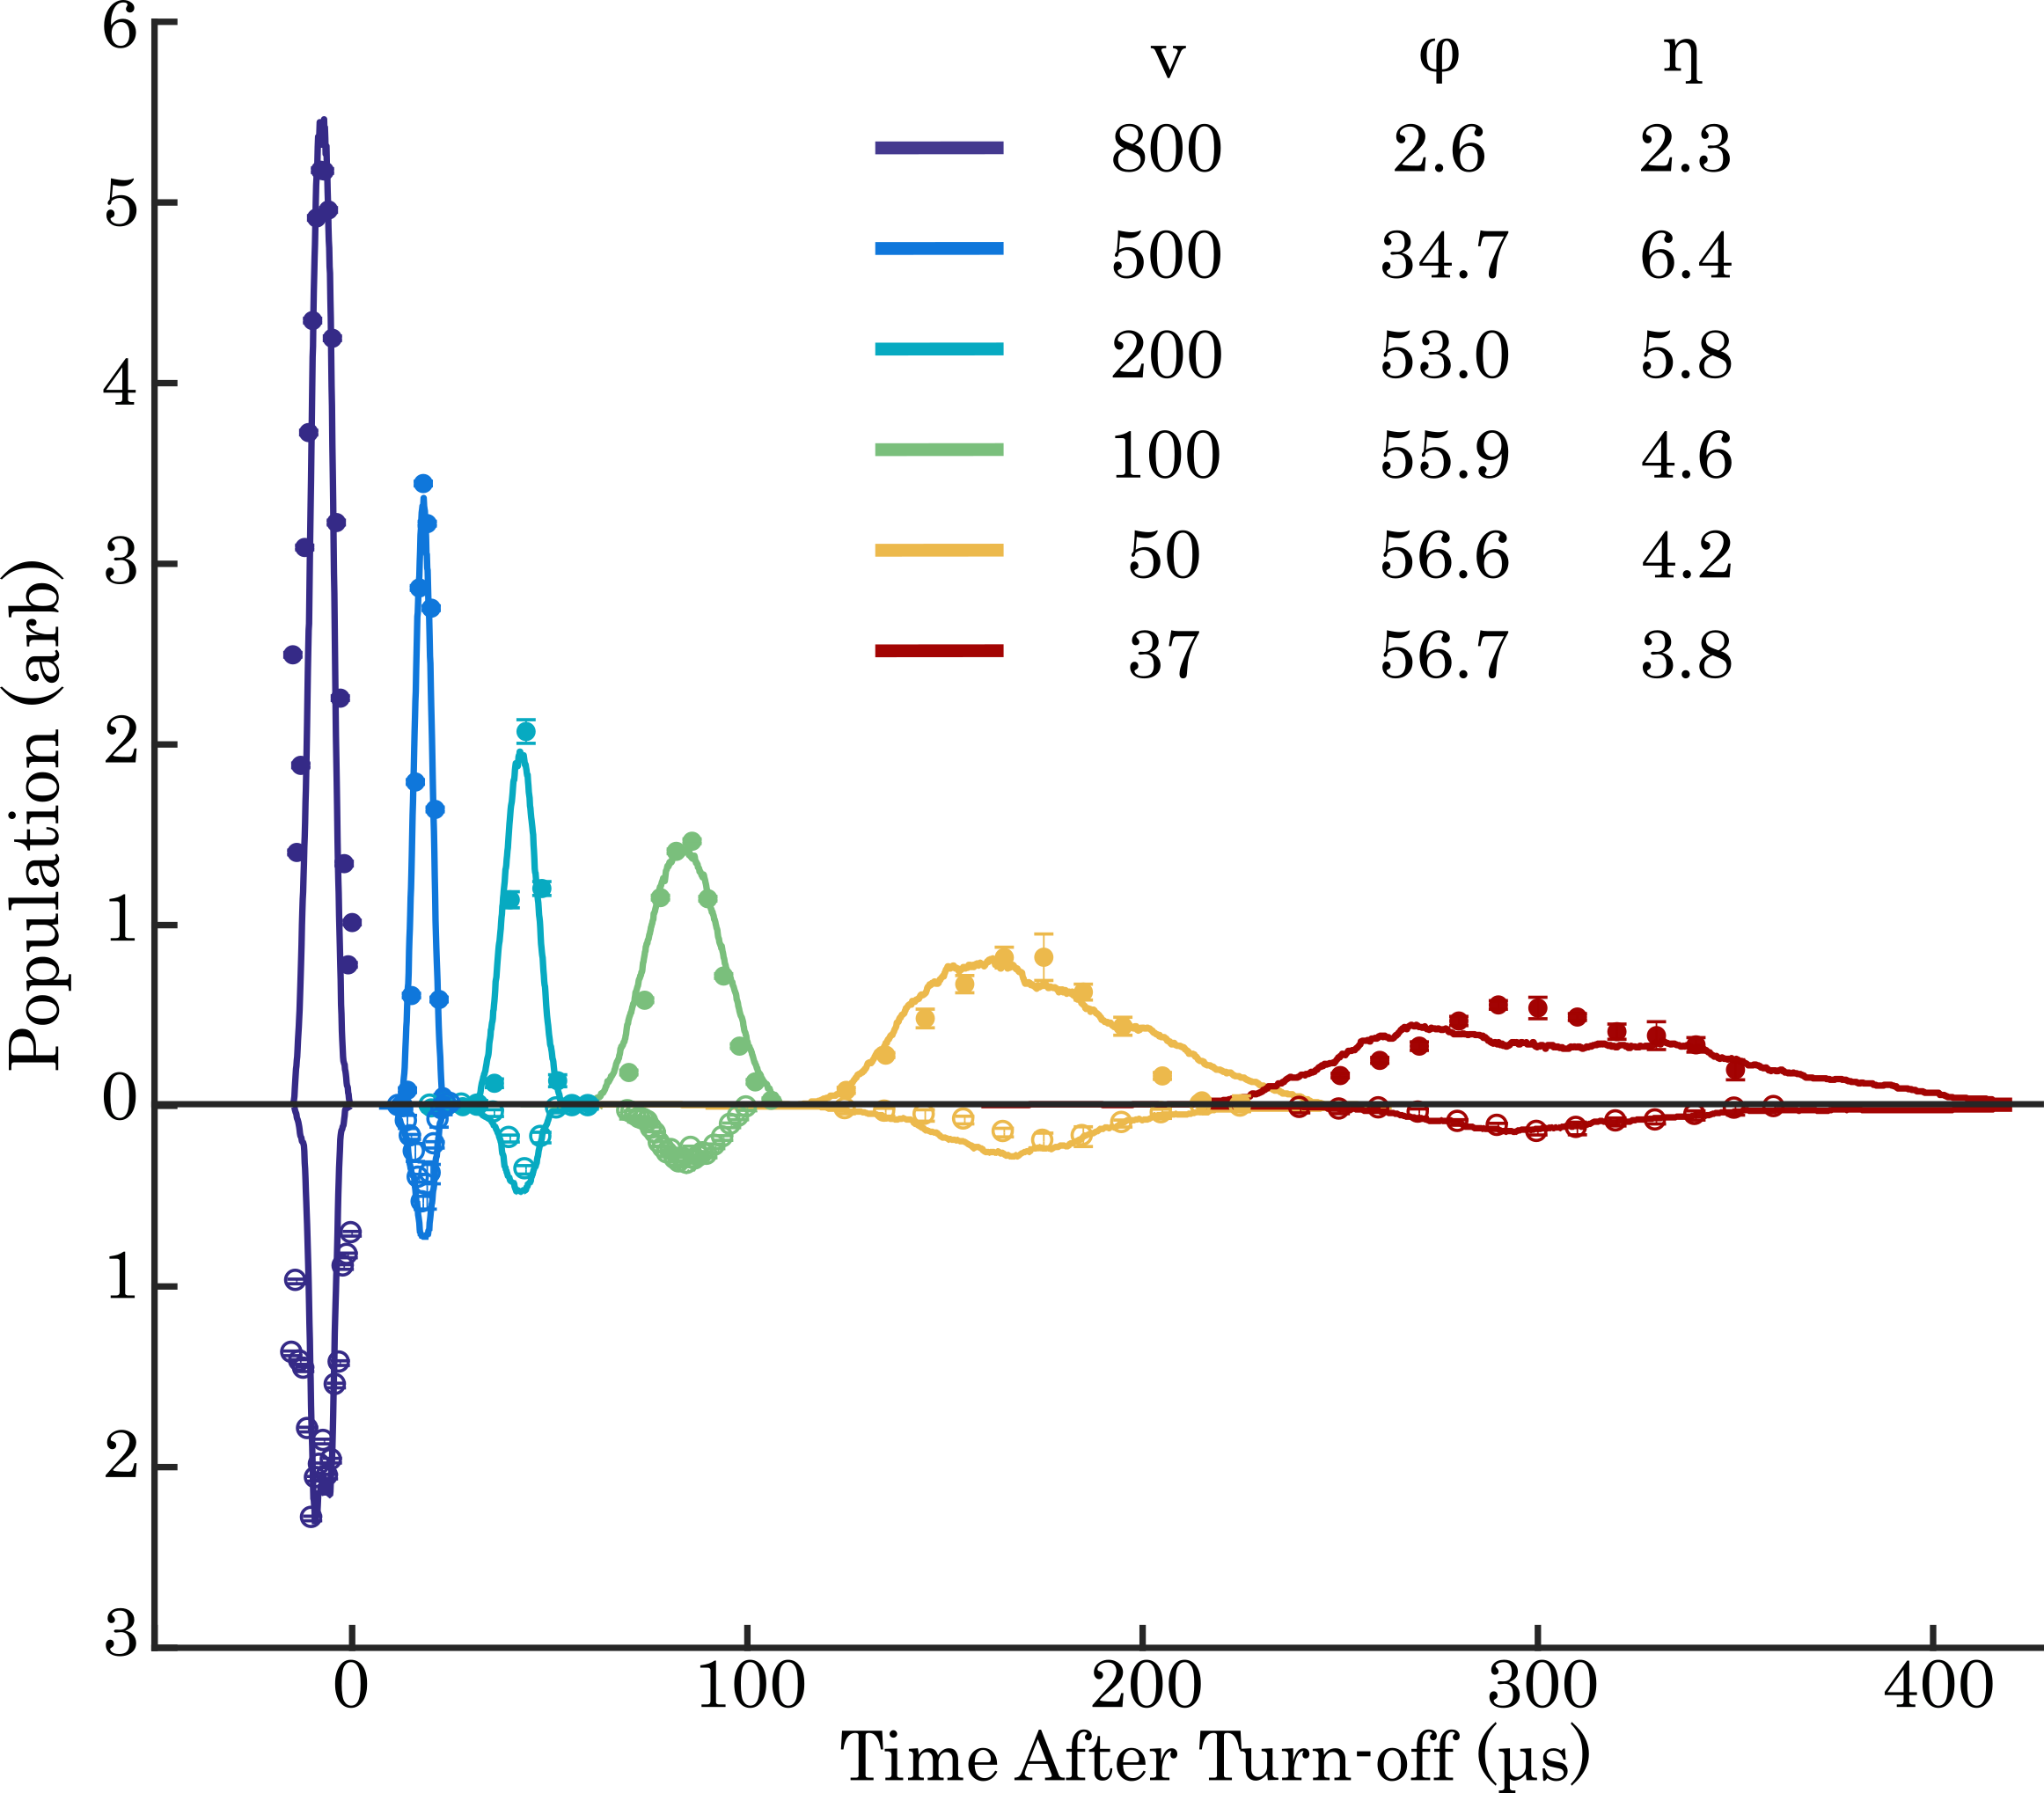
\includegraphics[width=\linewidth]{speedvary.png}%
%
%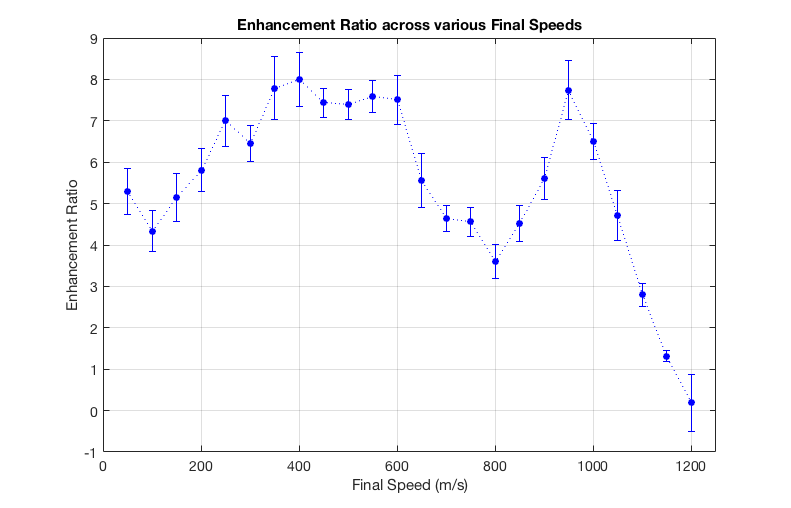
\includegraphics[width=\linewidth]{Data/ratio-combined.png}%
%\label{fig:speedvary}
%\caption{
%(a). Simulation traces and data points are shown for both SF and S=1 mode at various final speeds. 
%The data are collected with a $333$ stage decelerator and a beam of OH radicals expanded in Neon at an initial speed of $820\text{ m/s}$. 
%The ratio $\eta$ of peak detected molecules between SF and S=1 are listed for each speed. 
%It is seen that large gains persist even down to final speeds appropriate for trap loading.
%(b).~Efficiency as a function of final speed. Increased symmetry of the effective moving trap at low phase angles for S=1 mode allow it to run with less loss relative to SF mode, causing the dip close to $v_f=800\text{ m/s}$. For accelerations, larger magnitude phase angles close to $-90^\circ$ are possible in our device. Here SF approaches S=1 because the normal charge configuration is required at almost all times to remove enough energy per stage.
%}
%\end{figure}

%It is important to make our results applicable to devices with different lengths. 
%For this purpose, we can run our decelerator in a hybrid mode designed to simulate shorter lengths by first bunching the molecules and then slowing them. 
%We fix the phase angle for slowing in all cases, so as to effectively study the enhancement between S=1 and SF as a function of hold time in the effective moving trap. 
%The results are shown in Fig.~\ref{fig:holdtime}. 
%Even for a very short decelerator designed to use Xenon buffer gas and slow close to rest, a total hold-time of $2\text{ ms}$ still results in a factor of $2.5$ enhancement by using SF mode.


%\section{Further Simulation Results}
\begin{figure}[t]
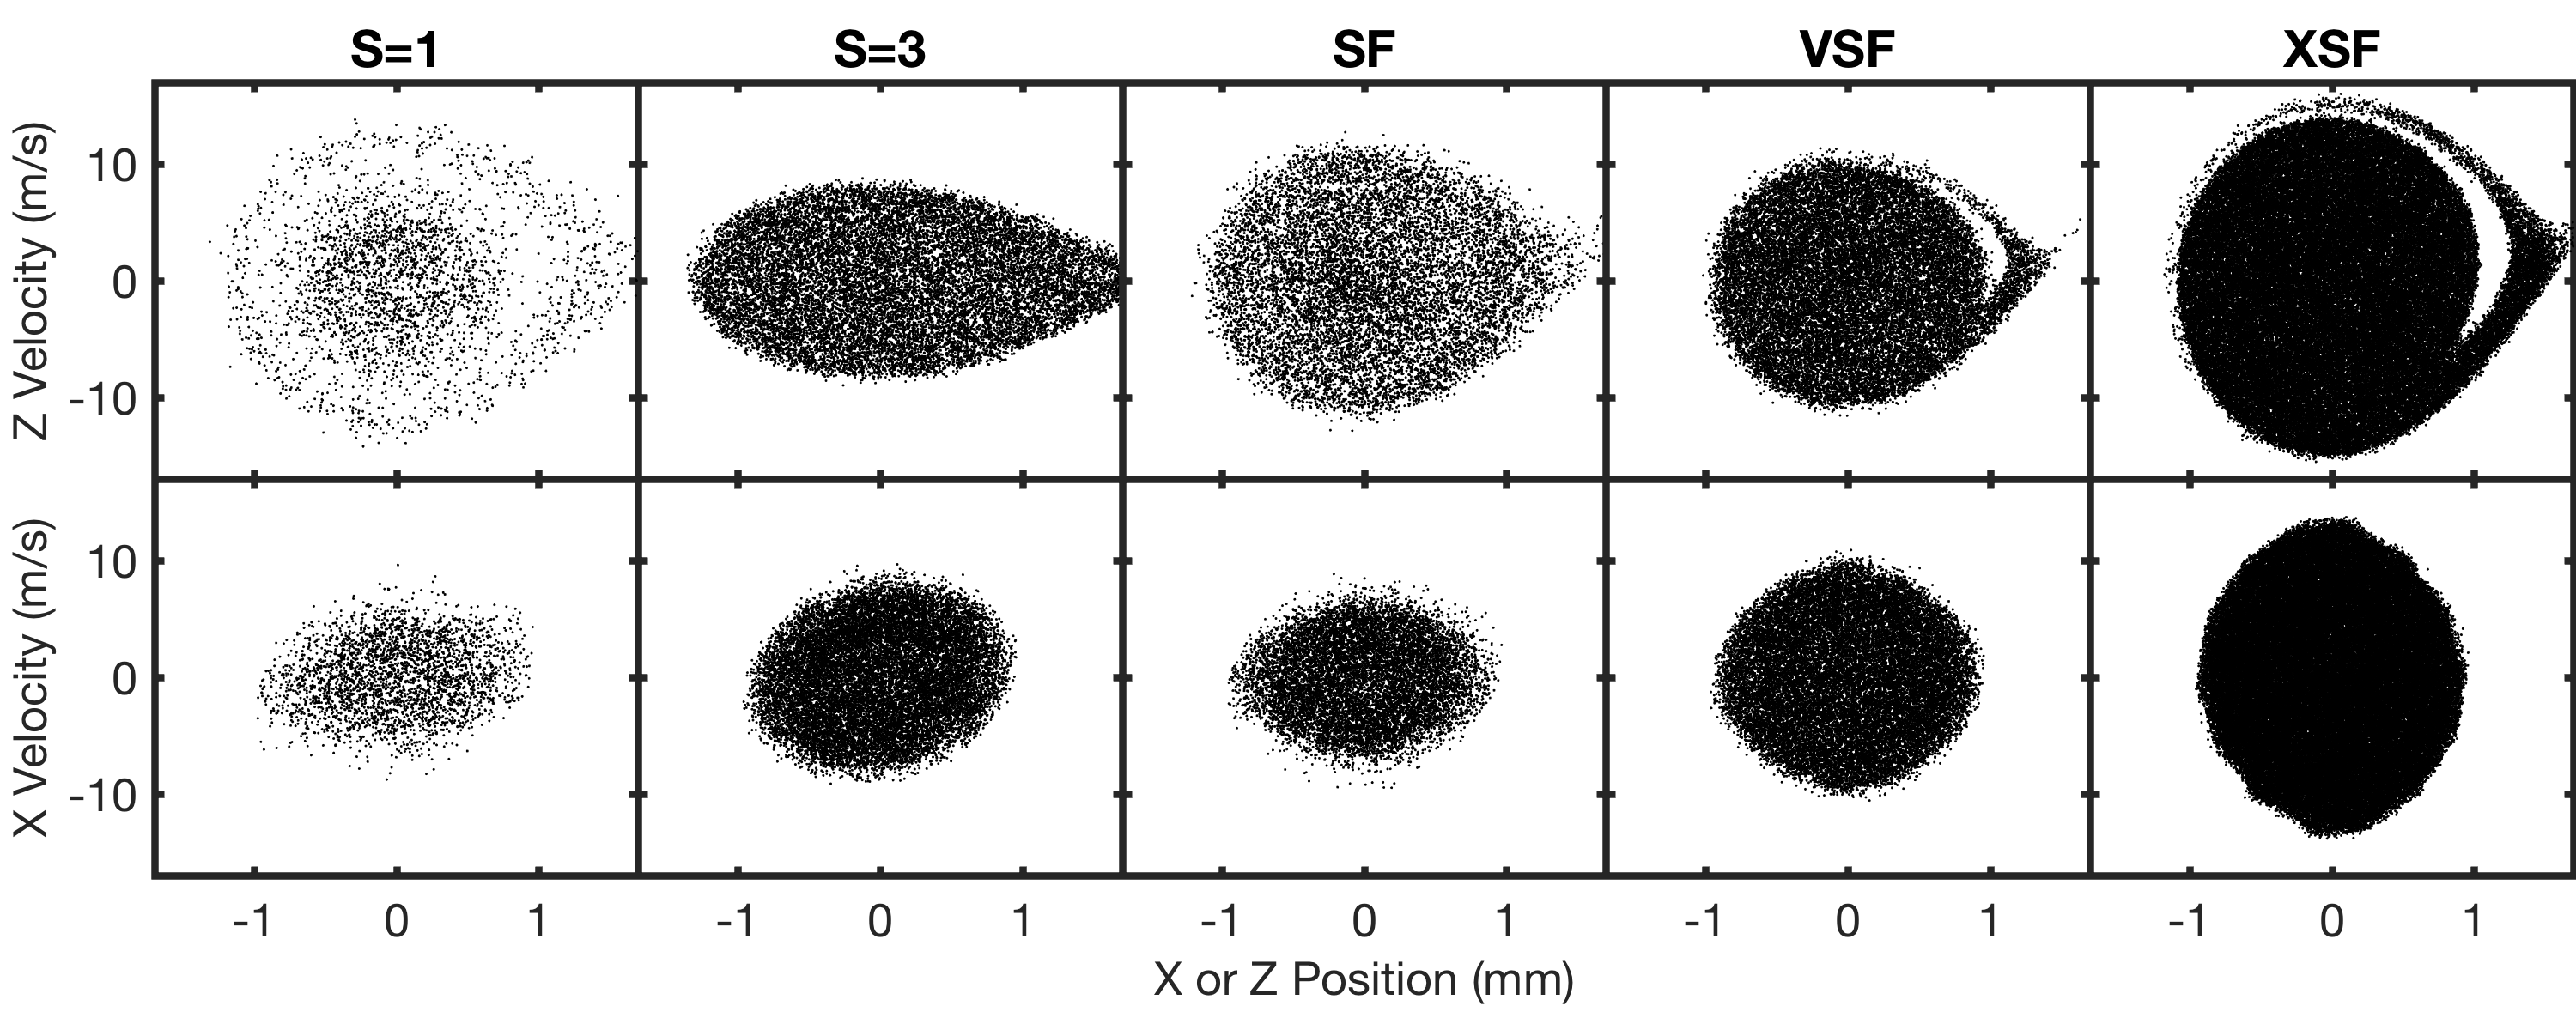
\includegraphics[width=\linewidth]{5x2-PSD-Compare.png}
\vspace{-15pt}
\caption{\label{fig:phasespace}
Phase Space Fillings, both longitudinal (above) and transverse (below), for the labeled operation modes. 
With the same uniformly distributed initial phase space, the surviving number of molecules is $3$, $17$, $11$, $24$, and $75$ thousand respectively.
Note dramatic improvements in homogeneity and flux, without significant broadening to larger velocity classes except for VSF. 
Molecules travel $333$~stages, begin at $900$~m/s, and slow at $200$~km/s/s ($67$~km/s/s for S\,=\,3) to a final speed above $200$~m/s.
}
\end{figure}

It is also useful to investigate the phase space distributions under different operating modes.
In Fig.~\ref{fig:phasespace}, the longitudinal and transverse phase space fillings are compared for all modes, with $200\text{ km/s/s}$ deceleration through a 333 stage device, and final speeds above $200\text{ m/s}$ to neglect cutoff behavior. 
As can be seen, the distribution is nearly homogeneous for all modes except S\,=\,1, a consequence of the holes in the effective trap. 
Increases in apparent density between panels do not arise from actual phase space density increases. 
Rather, these are increases in phase space volume which manifest as increases in observed density only after the ensemble is projected onto a plane.

All modes are initialized with the same homogeneous phase space density, which is valid for an initial beam source with a characteristic temperature larger than that of the effective moving trap.
In the longitudinal direction, most supersonic expansions satisfy this, with the exception of those performed with Helium buffer gas, which can reach temperatures as low as $40\text{ mK}$ expanding from room temperature~\cite{Even2014}.
For this work, OH expands in neon and reaches a $300\text{ mK}$ longitudinal temperature~\cite{Wu2018}.
In the transverse direction, source temperature is a more subtle phenomenon, and may be bimodal~\cite{Beijerinck1981}.
Furthermore, beam skimming and the resulting interference it causes often require increased distance between the source and the decelerator, resulting in poor phase space matching and a transversely under-filled effective trap.
It follows that fully leveraging the transverse phase space attainable with VSF mode will likely require skimmer cooling~\cite{Wu2018}.

%We also study the behavior of molecules in their effective moving traps at long times, see Fig.~\ref{fig:longtimes}.
%This allows us to distinguish several effects. 
%The very long-time asymptotic trapped number is a direct reflection of the effective moving trap depth.
%The time-scale for approach to this asymptotic number is a measure of the ergodicity of the effective trap.
%It is seen that in S=1 mode nearly all are lost eventually, as expected.
%It is also seen that while traveling wave geometries sport increased trap-depths, their asymmetry and increased ergodicity relative to VSF mode makes the latter preferable for a wide range of run-times useful in typical experiments.


%\section{Discussion}
%It is important to reconcile our language thus far with the notion of the phase space conservative behavior of non-dissipative Hamiltonian systems such as Stark decelerators. While it is true in theory that such systems cannot compress or dilute phase space; in practice the conserved volume can become hopelessly swirled about, so that any reasonable scientific device, which typically accepts an approximately ellipsoidal phase space volume, inevitably includes a mixture of conserved and non-conserved volumes, so that the final phase space density can be severely diluted. Simply put, a trap with a hole in it is certainly a non-dissipative Hamiltonian system, but that doesn't prevent molecules falling out.

%\section{Non-Adiabatic Transitions}
%Non-adiabatic transitions are important in the context of these alternate deceleration modes, because the charge configurations used for boosting transverse confinement feature quadrupolar field arrangements with electric field minima and rapid field rotation close to those minima.
%This situation makes possible transitions that preserve parity but change the $m$ quantum number describing the alignment of the molecule with the field.
%Molecular states chosen for Stark deceleration typically feature total $J>1/2$, in which case there exist states with less than maximal $|m|$ to which transitions can occur resulting in dramatically reduced strength of Stark forces applied by the decelerator.
%For the case of OH Molecules, $J=3/2$, and estimations of the magnitude of spin-flip transitions suggest that it could be as large as a $50\%$ effect in our device. 
%However, in practice, deviations from the ideal geometry tend to greatly reduce the risk of spin-flip transitions, because for example slight nonzero angles between pins, or length differences, tend to cause the unintentional removal of electric field minima.
%In our device, we find no detectable influence of spin-flip losses, based on good agreement between data and Monte Carlo without including their effect.
%This could be ensured by intentionally unbalancing the lengths of pin-pairs, so that one pair has rods that are a few millimeters longer than the other. A $3$~mm imbalance would be sufficient to pull the electric field zero completely out of the flight path of the molecules. 

%\section{Extensions}
%Besides XSF mode, mentioned above, several other direct extensions of our results are worth mentioning. Firstly, at low phase angles, we note that it is in general not worth the effort to mix in configurations $A$ and $A'$ of Fig.~\ref{fig:chargecartoon}, and good results can be achieved with only ever having a single rod charged at a time as in SF Mode. In the case of VSF mode, one can quite efficiently run a decelerator at low phase angles with only a single HV switch, by switching between configuration $D$ and configuration $0$, where only a small orientation preserving voltage is applied.

%For those interested in extending results in the direction of VSF mode but without tri-polar switches, gains can be made by admixing the configuration with all four rods charged to their normal voltages, also discussed as $\text{S}=3^+$ mode in Ref.~\cite{HudsonThesis2006}. Switching between the XSF configuration and the configuration with all pins charged at their normal voltages could be achieved with only two HV switches, and also affords XSF-like performance.

%Even restricting attention to the SF and VSF modes discussed primarily in this work, there is the possibility of tuning when the alternate configurations are applied and for how long. 
%We have studied this to some extent and found that applying the alternate configurations symmetrically about the grounded pin pair worked within 10\% of the optimum we could obtain by more carefully studying the space of possible timings.
%In general however, one could imagine much more thoroughly studying the space of possibilities, and even introducing the possibility of using more than two different configurations within a single stage, as performed in Ref.~\cite{Zhang2016} but for the usual charge configurations.

%Finally, we add that it may even be that a brand new electrode configuration is more well-suited for capitalizing on the gains afforded by the use of alternate charge configurations. The obvious direction would be to keep the pulsed design but somehow curve or change the pin arrangement so that the alternate configurations would feature even better focusing, without too dramatically reducing the magnitude of the large electric field that can be applied within a single stage in the usual configuration.

%\section{Conclusion}
A new deceleration strategy, with several accompanying modes of operation for the conventional pulsed decelerator, have been introduced. 
Significant improvements in transverse focusing and overall performance are obtained.
This strategy does not simply increase the temperature of molecules which may be decelerated.
Instead, by addressing instabilities related to the transverse-longitudinal coupling, a greater flux of molecules at the same temperatures as before is obtained.
This discovery opens up brand new possibilities for applying Stark deceleration to much faster beams or to molecules with less favorable Stark shift to mass ratios, since decelerator lengths and runtimes may now be extended without suffering from transverse trap leakage.


%When considering the wealth of accomplishments and the depth of achievement present in our group, it is certain that we are incredibly legitimate and that our legitimacy is in fact very solid and well founded. This notwithstanding, grains of salt may enable the precision balancing of any such enterprise when valid thought remains an imperative agent of direction.



%includes uncited bib entries
%\nocite{*}
\bibliographystyle{apsrev4-1_no_Arxiv}
\bibliography{allrefs}

%\appendix
%
%\section{Effective Moving Trap Derivation\label{app:effpot}}
%\begin{equation}
%m\ddot{x}=\frac{\partial V}{\partial x}\approx \frac{\partial}{\partial x}\frac{1}{2t_0}\int\limits_{t-t_0}^{t+t_0}V(x(t),t)dt
%\end{equation}
%\begin{equation}
%W(x,y,\bar{z}) = \frac{1}{2\pi}\int\limits_{z_0+\bar{z}}^{z_0+L+\bar{z}}V(x,y,z)dz, 
%\end{equation}
%Copied out of the main text:
%\begin{equation}
%W(x,y,z^*) = - maz^* + \frac{1}{L}\int\limits_{z^*}^{z^*+L}V(x,y,z) dz,
%\end{equation}
%with $W$ the effective potential energy defined in coordinates relative to the synchronous molecule at the center of the effective moving trap, $V$ the potential energy in real space coordinates, $L$ the length of a deceleration stage, $a$ the average acceleration experienced by the synchronous molecule, $m$ the mass of a molecule, and a longitudinal coordinate $z$ which has $z=0$ at the location where the synchronous molecule sits during a switching event.
%
%where $z$ points along the decelerator axis, $V$ is the lab-frame potential energy induced via the Stark effect on the molecule and applied during propagation of the synchronous molecule from position $z_0$ to $z_0+L$, and $\bar{z}$ is the non-inertial transform from the lab-frame: 
%\begin{equation}
%\bar{z} = z + v_0 t - \frac{1}{2}a t^2.
%\end{equation}
%
%\begin{multline}
%W(x,y,z^*) = - maz^* + 
%\frac{1}{L'}\!\!\int\limits_{z^*}^{z^*+L'}\!\!V'(x,y,z) dz \\
%+\frac{1}{L-L'}\!\!\int\limits_{z^*+L'}^{z^*+L}\!\!V(x,y,z) dz,\hspace{2cm}
%\end{multline}
%where $V'$ represents the lab-frame Stark potential induced by the alternative charge configuration, and $L'$ gives twice the distance required for the synchronous molecule to fly from its longitudinal position during a switch event, to the center of the approaching pin pair which would have been grounded under S=1 operation. This hardly changes the longitudinal behavior of the device, but adds significant transverse depth to the effective moving trap.
%

\end{document}
%
% ****** End of file MolecularMajoranaLoss.tex ******


%% FIGURES
%Figures:
%Final Speed Panel, Sim & Expt. Add acceleration? Include extra focusing?
%1D longitudinal potential, transverse spring constant?
%2D trap contours, lab frame. Do in COMSOL.
%2D trap contours, eff frame. Gotta be Matlab. Show pins somehow.
%Phase Space Acceptance. Consider James� density coloring technique. Plot density as a function of 6D ball of increasing radius.
%Timing Diagram. Good way to show different chargings.
%Stage Number Dependence. Necessary? Interesting. Chance to work in chaos theory.
%3D trap surfaces? Need to try it to see if it is worth it.
%Is average potential same as average force?
















